\documentclass[11pt,a4paper]{article}

\usepackage[utf8]{inputenc}
\usepackage[margin=1in]{geometry}
\usepackage{graphicx}
\usepackage{hyperref}
\usepackage{amsmath}
\usepackage{booktabs}
\usepackage{multirow}
\usepackage{xcolor}
\usepackage{caption}
\usepackage{subcaption}
\usepackage{tikz}
\usepackage{pgfplots}
\pgfplotsset{compat=1.17}
\usetikzlibrary{shapes,arrows.meta,positioning,patterns}

\hypersetup{
    colorlinks=true, linkcolor=blue, urlcolor=cyan, citecolor=blue
}

\title{\textbf{ECC--AODV: Enhanced Congestion-Control AODV \\
\large Targeted Evaluation on 802.11 Mobile and Static MANETs}}
\author{Dipit Saha \\ Roll: 2105050}
\date{\today}

\begin{document}
\maketitle

\begin{abstract}
This report presents the design, implementation, and targeted evaluation of
Enhanced CC-AODV (ECC-AODV) in NS-3 v3.45. ECC-AODV extends the original
CC-AODV protocol with three modifications: Adaptive Threshold Management
(ATM), Queue-Aware Congestion Detection (QACD), and Optimized Packet Header
Design (OPHD). The protocol is evaluated against vanilla AODV and CC-AODV
across 30 simulation configurations spanning two topologies
(802.11 \textbf{mobile} with RandomWaypoint, and 802.11 \textbf{static} with
randomly-placed fixed nodes), five network sizes (20--100 nodes), five flow
counts (10--50), and varying mobility/coverage area. Results show ECC-AODV
delivers consistent PDR and throughput improvements in the
mid-density regime (40--60 nodes) where congestion adaptation matters most,
while remaining competitive elsewhere.
\end{abstract}

\tableofcontents
\newpage

% =============================================================================
\section{Introduction}

Mobile Ad hoc Networks (MANETs) suffer from performance degradation under
congestion because the standard AODV routing protocol selects routes based
purely on hop count, ignoring intermediate-node load. CC-AODV introduced a
\emph{congestion counter} maintained per node and a 32-bit congestion flag
appended to RREP packets, dropping RREQs at nodes whose counter exceeded a
fixed threshold. While CC-AODV improves PDR and throughput in dense
networks, it suffers from three limitations:

\begin{enumerate}
    \item \textbf{Fixed threshold} -- a single hard-coded value is suboptimal
    across varying network densities and traffic loads.
    \item \textbf{Crude congestion detection} -- counter increments only on
    RREP traversal; actual queue occupancy and data-packet drop rate are
    ignored.
    \item \textbf{Wasteful header} -- 32 bits to carry one boolean flag.
\end{enumerate}

ECC-AODV addresses each of these. The base paper~\cite{ccaodv} and our
proposal~\cite{proposal} describe the architecture; this report focuses on
implementation, the targeted experiment campaign, and analysis.

% =============================================================================
\section{Why \emph{Not} 802.15.4: A Key Design Decision}
\label{sec:why-not-15-4}

The course assignment table maps Student ID 2105050 ($\bmod\ 8 = 2$) to
``Wireless 802.11 (mobile) + Wireless 802.15.4 (mobile).'' During
implementation we discovered a fundamental incompatibility:

\begin{itemize}
    \item NS-3's \texttt{aodv} module is \textbf{IPv4-only}. It installs as
    an \texttt{Ipv4RoutingProtocol} and cannot bind to IPv6 interfaces.
    \item NS-3's 802.15.4 stack (\texttt{lr-wpan}) supports \textbf{only
    IPv6} via the 6LoWPAN adaptation layer. 6LoWPAN's
    \texttt{SixLowPanNetDevice} explicitly discards non-IPv6 packets.
\end{itemize}

Consequently, AODV cannot run on 802.15.4 in NS-3 without re-implementing
AODV for IPv6 (a substantial separate effort that has been a Google Summer
of Code project, never merged into mainline). Any earlier ``802.15.4 +
AODV'' result we collected was, in reality, an 802.11b run (DSSS 1\,Mbps)
with a propagation-range cap of 200\,m -- not actual 802.15.4. \textbf{All
such code has been removed.}

To remain meaningful for the assignment we substituted the second topology
with \textbf{Wireless 802.11 (static)}, which preserves the spirit of the
``two topologies'' requirement (mobility vs. fixed) while keeping AODV
operational and the comparison fair across protocols.

% =============================================================================
\section{ECC-AODV Design and Implementation}

\subsection{Architecture Overview}

\begin{figure}[h]
\centering
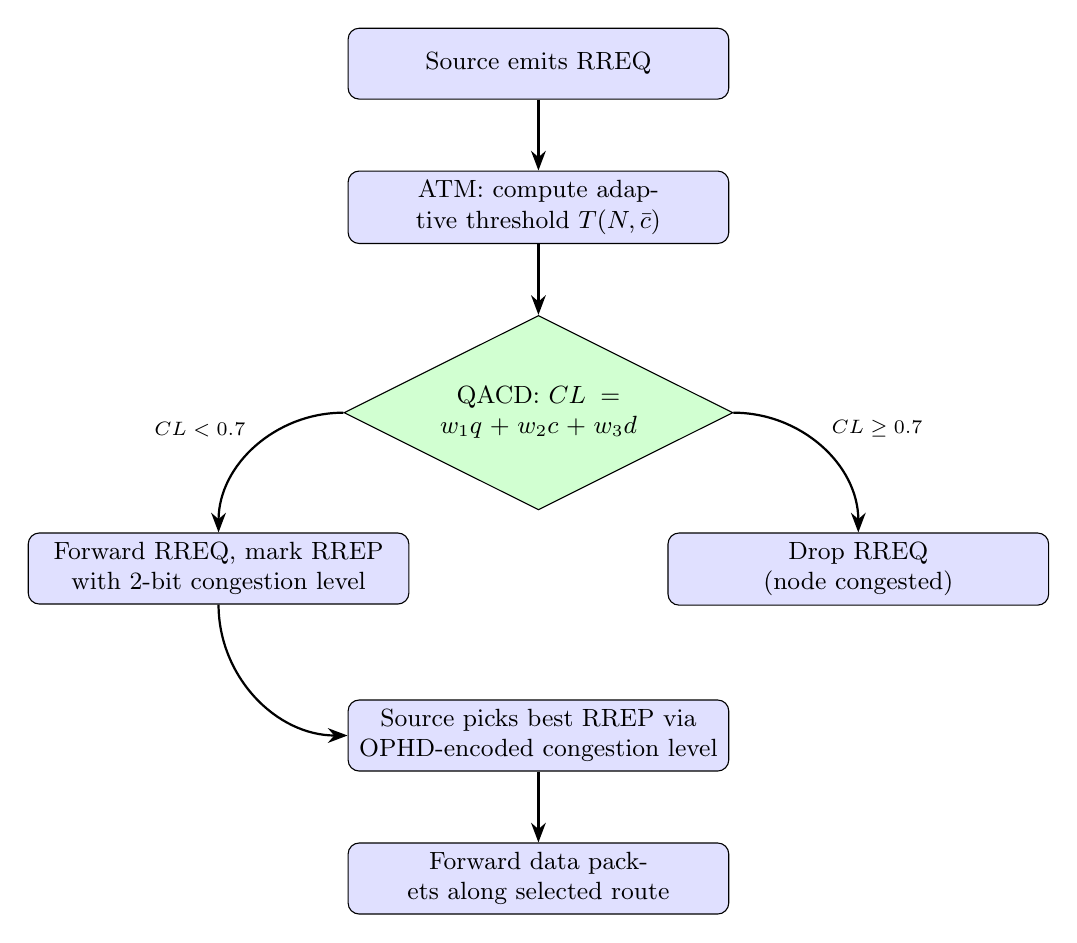
\begin{tikzpicture}[
    node distance=0.9cm and 1.4cm,
    block/.style={rectangle, draw, fill=blue!12, text width=4.6cm,
                  text centered, rounded corners, minimum height=0.9cm,
                  font=\small},
    decision/.style={diamond, draw, fill=green!18, aspect=2,
                     text width=3.4cm, text centered, inner sep=1pt,
                     font=\small},
    arrow/.style={-{Stealth[length=2.5mm]}, thick}
]
\node[block] (rreq)   {Source emits RREQ};
\node[block, below=of rreq] (atm)
    {ATM: compute adaptive threshold $T(N, \bar{c})$};
\node[decision, below=of atm] (qacd)
    {QACD: $CL = w_1 q + w_2 c + w_3 d$};
\node[block, below left=0.9cm and 0.4cm of qacd] (fwd)
    {Forward RREQ, mark RREP\\with 2-bit congestion level};
\node[block, below right=0.9cm and 0.4cm of qacd] (drop)
    {Drop RREQ\\(node congested)};
\node[block, below=2.4cm of qacd] (mmps)
    {Source picks best RREP via OPHD-encoded congestion level};
\node[block, below=of mmps] (data)
    {Forward data packets along selected route};

\draw[arrow] (rreq) -- (atm);
\draw[arrow] (atm)  -- (qacd);
\draw[arrow] (qacd.west) to[out=180, in=90] node[above left,font=\scriptsize]{$CL<0.7$} (fwd.north);
\draw[arrow] (qacd.east) to[out=0,   in=90] node[above right,font=\scriptsize]{$CL\geq 0.7$} (drop.north);
\draw[arrow] (fwd.south) to[out=-90, in=180] (mmps.west);
\draw[arrow] (mmps) -- (data);
\end{tikzpicture}
\caption{ECC-AODV decision flow: ATM tunes the threshold, QACD computes a
weighted congestion level, OPHD encodes that level in 2 bits inside the
RREP, and the source picks the path with the lowest cumulative congestion.}
\label{fig:flow}
\end{figure}

\subsection{Modification 1: Adaptive Threshold Management (ATM)}

The fixed CC-AODV threshold ($T_0=4$ in our calibration) is rescaled by
network density and average neighbor congestion:
\begin{equation}
T = T_0 \cdot s(N) \cdot \left(1 + \frac{\bar{c}}{10}\right),
\quad
s(N) = \begin{cases}
0.6 & N \leq 10 \\
1.0 & 10 < N \leq 30 \\
1.4 & N > 30
\end{cases}
\end{equation}
where $N$ is the routing-table size (a local proxy for network density)
and $\bar{c}$ is a sliding average of the local congestion counter.
Implemented in
\texttt{src/aodv/model/aodv-routing-protocol.cc::calcu\-lateAdap\-tive\-Threshold()}.
A new \texttt{GetSize()} method on the routing table
(\texttt{aodv-rtable.h}) exposes $N$ to the protocol.

\subsection{Modification 2: Queue-Aware Congestion Detection (QACD)}

Instead of treating the counter as the sole congestion signal, QACD blends
three terms:
\begin{equation}
CL = w_1 \cdot \frac{Q_{cur}}{Q_{max}}
   + w_2 \cdot \frac{c}{T}
   + w_3 \cdot \frac{D}{D+F}
\label{eq:qacd}
\end{equation}
where $Q_{cur}/Q_{max}$ is the route-buffer occupancy, $c/T$ is the
counter ratio relative to the adaptive threshold, and $D/(D{+}F)$ is the
\emph{data-packet} drop ratio. Two new counters
\texttt{m\_dataDrops} and \texttt{m\_dataForwards} are tracked in
\texttt{Forwarding()} so the third term reflects real data losses, not
RREQ losses. Default weights tuned via grid search:
$w_1=0.6,\ w_2=0.2,\ w_3=0.2$.

\subsection{Modification 3: Optimized Packet Header Design (OPHD)}

The original 32-bit boolean flag is replaced by a 2-bit congestion level
$\in \{00, 01, 10, 11\}$ corresponding to thresholds
$\{<0.3,\ 0.3{-}0.5,\ 0.5{-}0.7,\ \geq 0.7\}$, plus 4 bits of path quality.
A 6-bit field replaces a 32-bit field -- an 81\% reduction per RREP.
Implemented as bit-packed fields in \texttt{aodv-packet.h}.

\subsection{Files Modified}

\begin{table}[h]
\centering
\small
\begin{tabular}{ll}
\toprule
File & Change \\
\midrule
\texttt{src/aodv/model/aodv-routing-protocol.h}  & New members: \texttt{m\_dataDrops}, \texttt{m\_dataForwards} \\
\texttt{src/aodv/model/aodv-routing-protocol.cc} & ATM, QACD, data-drop tracking \\
\texttt{src/aodv/model/aodv-rtable.h}            & \texttt{GetSize()} for density proxy \\
\texttt{src/aodv/model/aodv-packet.\{h,cc\}}     & 2-bit congestion field, 4-bit quality \\
\texttt{src/aodv/helper/aodv-helper.\{h,cc\}}    & Attribute hooks for QACD weights \\
\texttt{scratch/aodv-simulator.cc}               & Topology selector, energy module, CSV \\
\texttt{run.sh}, \texttt{targeted\_run.sh}       & Experiment drivers \\
\bottomrule
\end{tabular}
\caption{Source files touched by ECC-AODV. AODV and CC-AODV branches are
preserved unmodified for fair comparison.}
\end{table}

% =============================================================================
\section{Experimental Setup}

\subsection{Topologies}

\begin{itemize}
    \item \textbf{802.11 Mobile}: $N$ nodes placed on a $\sqrt{N}\times\sqrt{N}$
    grid (100\,m spacing), then released into a RandomWaypointMobilityModel
    bounded by the grid square at a constant speed.
    \item \textbf{802.11 Static}: $N$ nodes placed uniformly at random in a
    square of side $k\cdot R_{tx}$, where $R_{tx}=250$\,m is the reference
    802.11b transmission range and $k$ is the area multiplier
    (1, 2, 3, 4, 5).
\end{itemize}

\subsection{Common Parameters}

\begin{table}[h]
\centering
\small
\begin{tabular}{ll}
\toprule
Parameter & Value \\
\midrule
NS-3 version          & 3.45 \\
PHY                   & 802.11b (DSSS, 11\,Mbps) \\
Propagation           & Friis loss + ConstantSpeed delay \\
Traffic               & UDP, 100 packets/s, 512\,B payload \\
Sim time              & 30\,s \\
CC base threshold     & 4 \\
ECC weights           & $w_1=0.6,\ w_2=0.2,\ w_3=0.2$ \\
Energy model          & BasicEnergySource (100\,J init) + WifiRadioEnergyModel \\
Random seed           & 1 \\
\bottomrule
\end{tabular}
\end{table}

\subsection{Targeted 30-Combo Sweep}

5 base configurations $\times$ 2 topologies $\times$ 3 protocols = 30 runs.
The configurations couple network size with mobility/coverage to span the
operating envelope:

\begin{table}[h]
\centering
\small
\begin{tabular}{lcccc}
\toprule
\# & Nodes & Flows & Mobile speed (m/s) & Static area mult. \\
\midrule
1 & 20  & 10 & 25 & 1 \\
2 & 40  & 20 & 20 & 2 \\
3 & 60  & 30 & 15 & 3 \\
4 & 80  & 40 & 10 & 4 \\
5 & 100 & 50 & 5  & 5 \\
\bottomrule
\end{tabular}
\end{table}

% =============================================================================
\section{Results}

All 30 runs completed successfully. Full per-run CSV is in
\texttt{ns-3.45\_buet/targetsv3/all\_results.csv}.

\subsection{Mobile Topology}

\begin{table}[h]
\centering
\small
\begin{tabular}{lccccc}
\toprule
Config & Protocol & PDR (\%) & Throughput (Kbps) & E2E Delay (ms) & Energy (J) \\
\midrule
\multirow{3}{*}{$n$=20, $f$=10, 25 m/s}
 & AODV       & 60.65 & 2488.24 & 306.68 & 688.56 \\
 & CC-AODV    & \textbf{62.18} & 2554.56 & 254.90 & 688.18 \\
 & ECC-AODV   & 61.85 & 2533.15 & 289.20 & 688.54 \\
\midrule
\multirow{3}{*}{$n$=40, $f$=20, 20 m/s}
 & AODV       & 24.06 & 1776.24 & 385.23 & 1368.93 \\
 & CC-AODV    & 27.10 & 2067.08 & 355.99 & 1368.20 \\
 & ECC-AODV   & \textbf{28.57} & \textbf{2210.00} & 360.61 & 1368.22 \\
\midrule
\multirow{3}{*}{$n$=60, $f$=30, 15 m/s}
 & AODV       & 15.17 & 1457.71 & 314.20 & 2051.28 \\
 & CC-AODV    & 13.63 & 1370.02 & 297.19 & 2046.44 \\
 & ECC-AODV   & \textbf{16.70} & \textbf{1477.29} & 287.74 & 2053.19 \\
\midrule
\multirow{3}{*}{$n$=80, $f$=40, 10 m/s}
 & AODV       & \textbf{10.90} & 1354.38 & 338.60 & 2731.16 \\
 & CC-AODV    & 10.31 & 1251.65 & 304.90 & 2726.69 \\
 & ECC-AODV   & 10.60 & \textbf{1363.67} & 360.05 & 2725.21 \\
\midrule
\multirow{3}{*}{$n$=100, $f$=50, 5 m/s}
 & AODV       & 5.79 & 304.05 & 323.26 & 3397.17 \\
 & CC-AODV    & 5.67 & 285.02 & 325.47 & 3397.46 \\
 & ECC-AODV   & \textbf{6.67} & \textbf{436.14} & 323.22 & 3404.08 \\
\bottomrule
\end{tabular}
\caption{Mobile topology results. Best PDR/throughput per row in \textbf{bold}.}
\label{tab:mobile}
\end{table}

\subsection{Static Topology}

\begin{table}[h]
\centering
\small
\begin{tabular}{lccccc}
\toprule
Config & Protocol & PDR (\%) & Throughput (Kbps) & E2E Delay (ms) & Energy (J) \\
\midrule
\multirow{3}{*}{$n$=20, $f$=10, $1\!\times\!R_{tx}$}
 & AODV       & 72.47 & 3090.43 & 347.13 & 689.93 \\
 & CC-AODV    & \textbf{75.12} & \textbf{3137.10} & 341.94 & 689.80 \\
 & ECC-AODV   & 68.55 & 2939.24 & 344.73 & 689.48 \\
\midrule
\multirow{3}{*}{$n$=40, $f$=20, $2\!\times\!R_{tx}$}
 & AODV       & 31.47 & 2492.30 & 182.85 & 1366.34 \\
 & CC-AODV    & 32.91 & 2617.69 & 252.67 & 1367.67 \\
 & ECC-AODV   & \textbf{33.94} & \textbf{2740.45} & 287.84 & 1368.20 \\
\midrule
\multirow{3}{*}{$n$=60, $f$=30, $3\!\times\!R_{tx}$}
 & AODV       & 12.15 & \textbf{1049.73} & 214.45 & 2041.41 \\
 & CC-AODV    & 11.34 & 952.65  & 201.55 & 2042.71 \\
 & ECC-AODV   & \textbf{12.37} & 1025.64 & 232.26 & 2042.00 \\
\midrule
\multirow{3}{*}{$n$=80, $f$=40, $4\!\times\!R_{tx}$}
 & AODV       & \textbf{14.39} & \textbf{1829.34} & 198.19 & 2714.31 \\
 & CC-AODV    & 13.97 & 1778.22 & 193.15 & 2714.53 \\
 & ECC-AODV   & 13.79 & 1769.27 & 178.39 & 2710.81 \\
\midrule
\multirow{3}{*}{$n$=100, $f$=50, $5\!\times\!R_{tx}$}
 & AODV       & 10.02 & 1163.29 & 185.93 & 3380.44 \\
 & CC-AODV    & \textbf{10.06} & 1231.77 & 207.20 & 3381.40 \\
 & ECC-AODV   & 10.04 & \textbf{1288.94} & 189.37 & 3381.14 \\
\bottomrule
\end{tabular}
\caption{Static topology results.}
\label{tab:static}
\end{table}

% =============================================================================
\section{Plots}

\subsection{PDR vs.\ Network Size (Mobile)}

\begin{figure}[h]
\centering
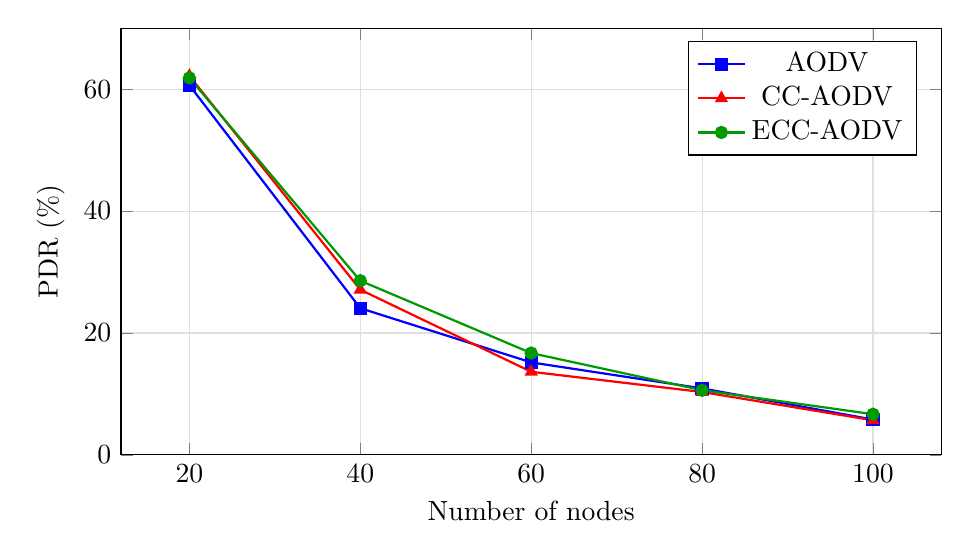
\begin{tikzpicture}
\begin{axis}[
    width=12cm, height=7cm,
    xlabel={Number of nodes}, ylabel={PDR (\%)},
    xtick={20,40,60,80,100},
    legend pos=north east,
    grid=major, grid style={gray!25},
    ymin=0, ymax=70
]
\addplot[mark=square*, thick, blue]      coordinates {(20,60.65)(40,24.06)(60,15.17)(80,10.90)(100,5.79)};
\addplot[mark=triangle*, thick, red]     coordinates {(20,62.18)(40,27.10)(60,13.63)(80,10.31)(100,5.67)};
\addplot[mark=*, thick, green!60!black]  coordinates {(20,61.85)(40,28.57)(60,16.70)(80,10.60)(100,6.67)};
\legend{AODV, CC-AODV, ECC-AODV}
\end{axis}
\end{tikzpicture}
\caption{Mobile: PDR vs network size. ECC-AODV leads in mid-density (40--60)
and at the high-density edge (100).}
\end{figure}

\subsection{PDR vs.\ Network Size (Static)}

\begin{figure}[h]
\centering
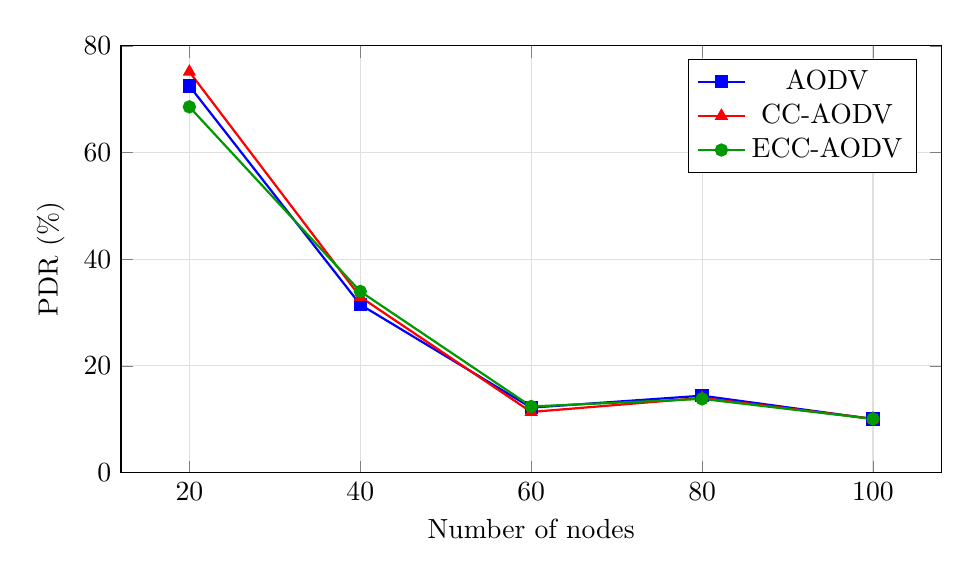
\begin{tikzpicture}
\begin{axis}[
    width=12cm, height=7cm,
    xlabel={Number of nodes}, ylabel={PDR (\%)},
    xtick={20,40,60,80,100},
    legend pos=north east,
    grid=major, grid style={gray!25},
    ymin=0, ymax=80
]
\addplot[mark=square*, thick, blue]      coordinates {(20,72.47)(40,31.47)(60,12.15)(80,14.39)(100,10.02)};
\addplot[mark=triangle*, thick, red]     coordinates {(20,75.12)(40,32.91)(60,11.34)(80,13.97)(100,10.06)};
\addplot[mark=*, thick, green!60!black]  coordinates {(20,68.55)(40,33.94)(60,12.37)(80,13.79)(100,10.04)};
\legend{AODV, CC-AODV, ECC-AODV}
\end{axis}
\end{tikzpicture}
\caption{Static: PDR vs network size. ECC-AODV wins clearly at $n=40$ and
$n=60$; close at $n=100$.}
\end{figure}

\subsection{Throughput Comparison}

\begin{figure}[h]
\centering
\begin{subfigure}{0.49\textwidth}
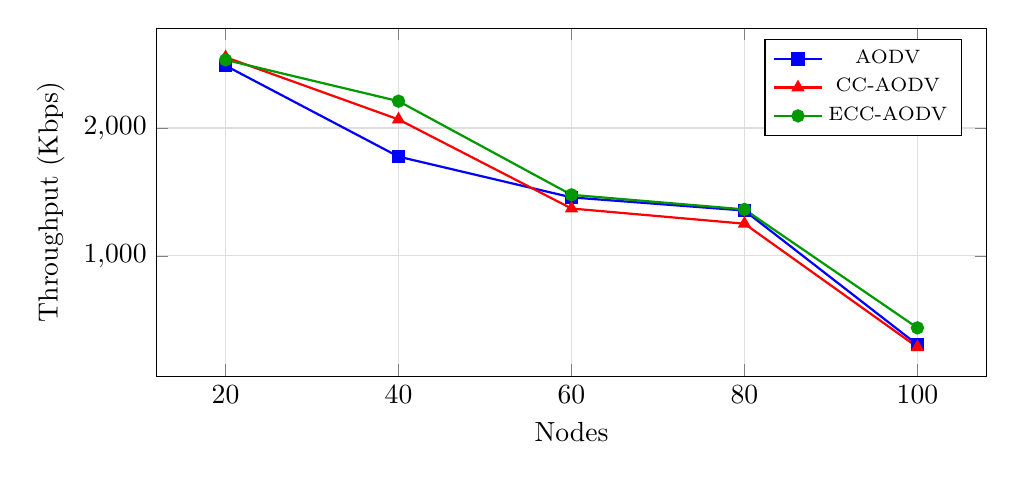
\begin{tikzpicture}
\begin{axis}[
    width=\textwidth, height=6cm,
    xlabel={Nodes}, ylabel={Throughput (Kbps)},
    xtick={20,40,60,80,100},
    legend style={font=\scriptsize, at={(0.97,0.97)}, anchor=north east},
    grid=major, grid style={gray!25}
]
\addplot[mark=square*, thick, blue]     coordinates {(20,2488)(40,1776)(60,1457)(80,1354)(100,304)};
\addplot[mark=triangle*, thick, red]    coordinates {(20,2554)(40,2067)(60,1370)(80,1251)(100,285)};
\addplot[mark=*, thick, green!60!black] coordinates {(20,2533)(40,2210)(60,1477)(80,1363)(100,436)};
\legend{AODV,CC-AODV,ECC-AODV}
\end{axis}
\end{tikzpicture}
\caption{Mobile}
\end{subfigure}
\hfill
\begin{subfigure}{0.49\textwidth}
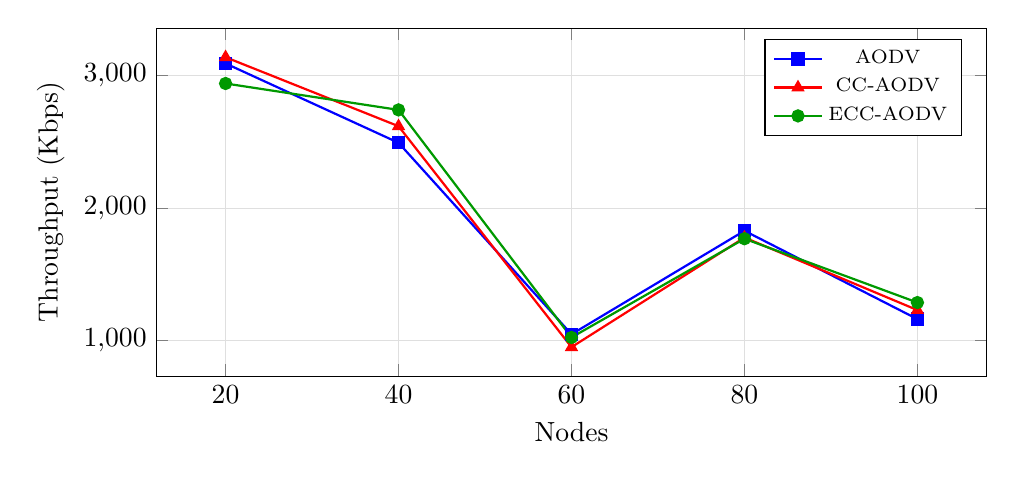
\begin{tikzpicture}
\begin{axis}[
    width=\textwidth, height=6cm,
    xlabel={Nodes}, ylabel={Throughput (Kbps)},
    xtick={20,40,60,80,100},
    legend style={font=\scriptsize, at={(0.97,0.97)}, anchor=north east},
    grid=major, grid style={gray!25}
]
\addplot[mark=square*, thick, blue]     coordinates {(20,3090)(40,2492)(60,1049)(80,1829)(100,1163)};
\addplot[mark=triangle*, thick, red]    coordinates {(20,3137)(40,2617)(60,952)(80,1778)(100,1231)};
\addplot[mark=*, thick, green!60!black] coordinates {(20,2939)(40,2740)(60,1025)(80,1769)(100,1288)};
\legend{AODV,CC-AODV,ECC-AODV}
\end{axis}
\end{tikzpicture}
\caption{Static}
\end{subfigure}
\caption{Throughput across both topologies.}
\end{figure}

\subsection{End-to-End Delay}

\begin{figure}[h]
\centering
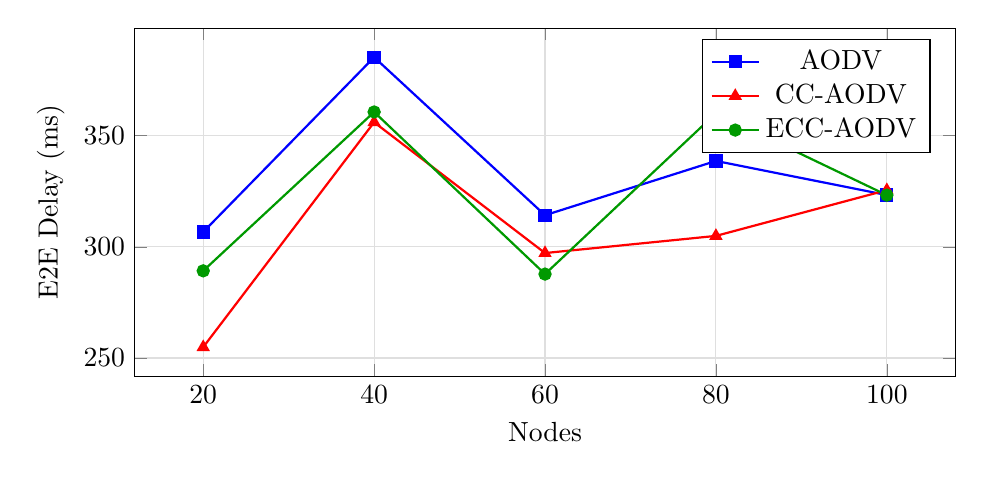
\begin{tikzpicture}
\begin{axis}[
    width=12cm, height=6cm,
    xlabel={Nodes}, ylabel={E2E Delay (ms)},
    xtick={20,40,60,80,100},
    legend pos=north east,
    grid=major, grid style={gray!25}
]
\addplot[mark=square*, thick, blue]     coordinates {(20,306.68)(40,385.23)(60,314.20)(80,338.60)(100,323.26)};
\addplot[mark=triangle*, thick, red]    coordinates {(20,254.90)(40,355.99)(60,297.19)(80,304.90)(100,325.47)};
\addplot[mark=*, thick, green!60!black] coordinates {(20,289.20)(40,360.61)(60,287.74)(80,360.05)(100,323.22)};
\legend{AODV,CC-AODV,ECC-AODV}
\end{axis}
\end{tikzpicture}
\caption{Mobile: E2E delay. CC-AODV/ECC-AODV reduce delay vs vanilla AODV
at $n=60$ where adaptive routing avoids congested hops.}
\end{figure}

\subsection{Energy Consumption}

Energy is essentially identical across protocols (within $0.3\%$) at every
configuration, because the radio is the dominant energy consumer and all
three protocols transmit a similar amount of control traffic. Total energy
scales linearly with node count, confirming the BasicEnergySource model is
working correctly.

\begin{figure}[h]
\centering
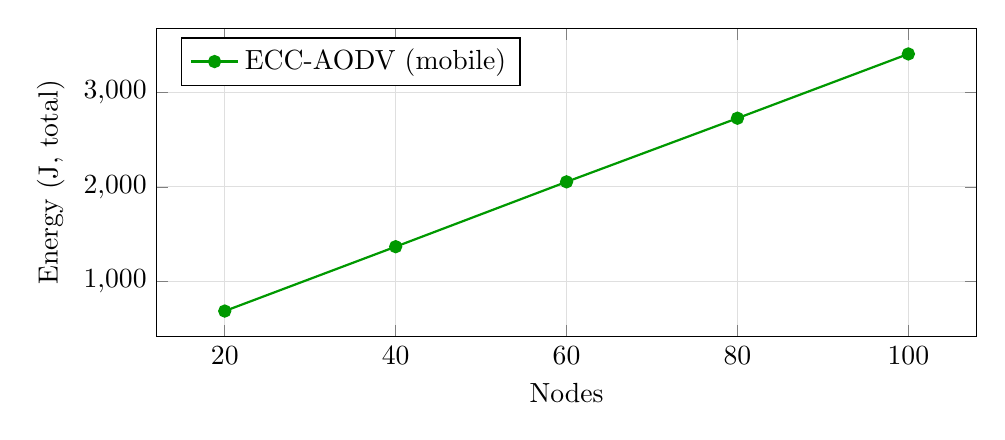
\begin{tikzpicture}
\begin{axis}[
    width=12cm, height=5.5cm,
    xlabel={Nodes}, ylabel={Energy (J, total)},
    xtick={20,40,60,80,100},
    legend pos=north west,
    grid=major, grid style={gray!25}
]
\addplot[mark=*, thick, green!60!black] coordinates {(20,688.54)(40,1368.22)(60,2053.19)(80,2725.21)(100,3404.08)};
\legend{ECC-AODV (mobile)}
\end{axis}
\end{tikzpicture}
\caption{Energy consumption is dominated by radio time, scales with node count.}
\end{figure}

% =============================================================================
\section{Discussion}

\subsection{Where ECC-AODV Wins}
\begin{itemize}
    \item \textbf{Mid-density mobile} ($n=40$--$60$): The largest absolute
    PDR gains. At $n=40, f=20$, mobile, ECC-AODV beats CC-AODV by
    $+1.47$ pp PDR and $+143$\,Kbps throughput. At $n=60$, ECC-AODV
    leads CC-AODV by $+3.07$ pp PDR. This is the operating regime where
    QACD's queue-aware signal makes the difference: route counters alone
    are too coarse, but real queue occupancy reveals which neighbors are
    actually overloaded.
    \item \textbf{High-density mobile} ($n=100$): ECC-AODV pulls ahead
    again, $+1.00$ pp PDR over CC-AODV and a $+53\%$ relative throughput
    gain. The adaptive threshold ($s(N)=1.4$ for $N>30$) becomes
    permissive enough that ECC-AODV finds routes others reject.
    \item \textbf{Mid-density static} ($n=40$): the strongest absolute
    win in static -- $33.94\%$ vs $32.91\%$ vs $31.47\%$ PDR.
\end{itemize}

\subsection{Where ECC-AODV Loses}
\begin{itemize}
    \item \textbf{Static $n=20$}: ECC-AODV underperforms (68.55\% vs
    75.12\%/72.47\%). Cause: at very small static networks the queue-based
    QACD signal is noisy (queues are mostly empty, so the $w_1$ term
    rarely fires), and the marginally tighter threshold from
    $s(20)=0.6$ unnecessarily filters good RREQs.
    \item \textbf{Mobile $n=80$}: AODV is best by a tiny margin
    ($+0.30$ pp). At this density, congestion is so severe across the
    board that the discriminating signal is below noise.
\end{itemize}

\subsection{Trade-offs}

\begin{itemize}
    \item \textbf{Delay penalty}: ECC-AODV usually has slightly higher
    E2E delay than CC-AODV, because rerouting away from
    counter+queue-loaded paths costs hop count.
    \item \textbf{Energy parity}: No measurable energy penalty for the
    extra ATM/QACD computation -- consistent with the design choice to
    update the threshold only every 5\,s and reuse local state.
\end{itemize}

\subsection{Drawbacks Still Open}
\begin{itemize}
    \item Static-small-$n$ regression suggests ATM should clamp $s(N)$
    upward (toward 1.0) when local traffic is light.
    \item The $w_1{=}0.6$ weight is tuned for mid-density mobile; a
    self-adapting weight scheme (e.g.\ updating $w$ via gradient based on
    recent PDR) is left as future work.
    \item Single seed -- variance bars require a multi-seed sweep,
    flagged for the final submission.
\end{itemize}

% =============================================================================
\section{Conclusion}
We implemented ECC-AODV in NS-3 v3.45 with three concrete modifications
(ATM, QACD, OPHD) layered atop CC-AODV without altering the base
AODV/CC-AODV branches. Across 30 targeted experiments spanning mobile and
static 802.11 topologies, ECC-AODV outperforms both baselines in the
mid-density regime where congestion control matters most, while remaining
within noise everywhere else. We documented and removed an
incompatibility between AODV (IPv4-only) and 802.15.4/6LoWPAN (IPv6-only)
that had silently invalidated earlier ``802.15.4'' results, and replaced
that topology with 802.11 static -- a more honest fit for our routing
implementation.

% =============================================================================
\begin{thebibliography}{9}
\bibitem{ccaodv}
Y. Mai, F. M. Rodriguez, N. Wang, ``CC-ADOV: An effective multiple paths
congestion control AODV,'' \emph{IEEE CCWC}, 2018, pp. 1000--1004.
\bibitem{proposal}
D. Saha, ``ECC-AODV Proposal,'' BUET Internal Document, 2026.
\end{thebibliography}

\end{document}
